\documentclass{oblivoir}
\usepackage{amsmath,amssymb,amsthm,kotex,mdframed,paralist,kswrapfig}

\newcounter{num}
\newcommand{\prob}
{\bigskip\noindent\refstepcounter{num}\textbf{문제 \arabic{num})}\par}

\newcommand{\subprob}
{\bigskip\noindent\textbf{추가문제 \arabic{num}-1)}\par}

\newcommand{\subprobb}
{\bigskip\noindent\textbf{추가문제 \arabic{num}-2)}\par}

\newcommand{\ans}{{\raggedleft\textbf{답 : (\qquad\qquad\qquad\qquad\qquad\qquad)}
\par}\bigskip\bigskip}


\newcommand\ga{\text{(가)}}
\renewcommand\na{\text{(나)}}


%%%
\begin{document}
\Large

\title{승재 14 - 6학년 2학기 - 07}
\author{}
\date{\today}
\maketitle
%\tableofcontents

\newpage

%
\prob
(가)의 0.3는 (나)의 \(\displaystyle\frac13\)과 같을 때 (가) : (나)를 가장 간단한 자연수의 비로 나타내고, 그 풀이과정을 쓰세요.
\begin{figure}[h]
\centering
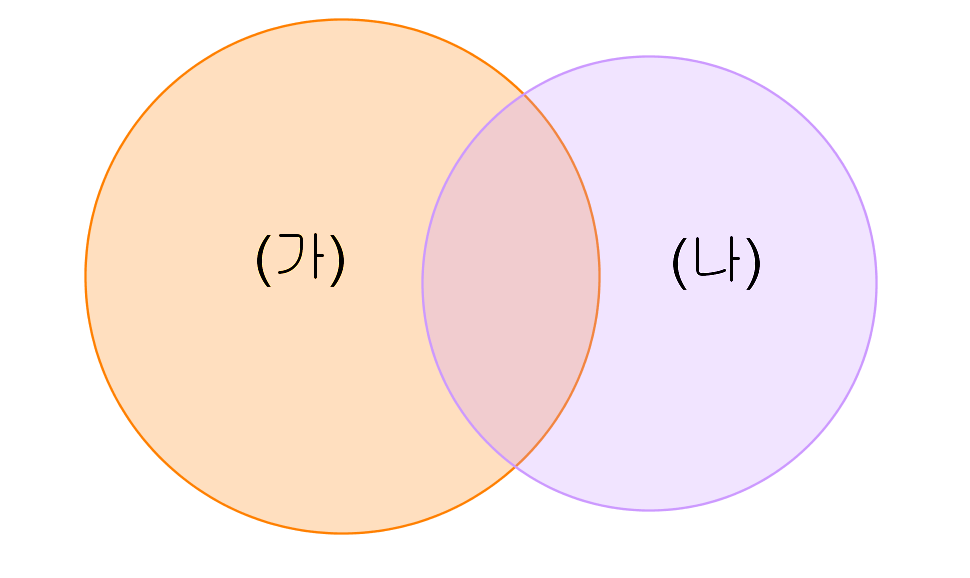
\includegraphics[width=0.5\textwidth]{venn}
\end{figure}
\begin{mdframed}
\textbf{풀이 : }
\vspace{0.3\textheight}
\end{mdframed}

\ans

\subprob
(가)의 \(\displaystyle\frac2{11}\)는 (나)의 0.22과 같을 때 (가) : (나)를 가장 간단한 자연수의 비로 나타내세요.

\subprob
(가)의 \(\displaystyle\frac34\)는 (나)의 0.85과 같을 때 (가) : (나)를 가장 간단한 자연수의 비로 나타내세요.

\newpage

%
\prob
(가) : (나)를 가장 간단한 자연수의 비로 나타내고 그 풀이과정을 쓰세요.
\[
\ga\times\frac18=\na\times2.7
\]
\begin{mdframed}
\textbf{풀이 : }
\vspace{0.3\textheight}
\end{mdframed}
\ans

\subprob
(가) : (나)를 가장 간단한 자연수의 비로 나타내세요.
\[
\ga\times\frac32=\na\times6.5
\]
\subprob
(가) : (나)를 가장 간단한 자연수의 비로 나타내세요.
\[
\ga\times2.4=\na\times\frac49
\]

\newpage

%
\prob
준호가 이번 시험에서 받은 국어, 영어, 수학 점수를 살펴보았더니, 국어 점수는 영어 점수의 \(\frac34\)이고 수학 점수는 영어 점수의 \(\frac{10}9\)이었습니다.
이 때, 국어 점수:수학 점수를 가장 간단한 자연수의 비로 나타내고, 그 풀이과정을 쓰세요.

\begin{mdframed}
\textbf{풀이 : }
\vspace{0.3\textheight}
\end{mdframed}
\ans

\textbf{(추가문제)} 만약 영어 점수가 72점이었다면, 국어와 수학 중 어떤 과목의 점수가 몇 점 더 높습니까?

\subprob
민희의 국어 점수는 영어 점수의 0.9이고 수학 점수는 영어 점수의 \(\frac9{11}\)입니다.
이 때, 국어 점수:수학 점수를 가장 간단한 자연수의 비로 나타내세요.

\subprob
상재의 국어 점수는 영어 점수의 0.85이고 수학 점수는 영어 점수의 \(\frac{13}{16}\)입니다.
영어 점수가 80점이라면 국어와 수학 중 어떤 과목의 점수가 몇 점 더 높습니까?

\end{document}